\chapter{Daten \& SQL}\label{ch:Lektion}
\section{Einführung}

\subsection{Was sind Daten?}

Der Begriff \enquote{Daten} ist der Plural von \textit{Datum} und kommt aus dem Lateinischen (\textit{datum} $=$ gegeben,
bzw. \textit{dare} $=$ geben). \enquote{Daten} bedeuten also im weitesten Sinne etwas \enquote{\textbf{Gegebenes}}, d.h. Angaben über Personen, Dinge oder Ereignisse. Beispiele von Daten sind:
\begin{itemize}
  \item \enquote{Mein Nachbar heisst Marco Odermatt.}
  \item \enquote{Aktuell findet an der KLW Unterricht statt.}
  \item \enquote{Das Billett von Zürich nach Winterthur kostet CHF 6.80.}
  \item \enquote{Das Logo der KLW besteht aus blauen und roten Farben.}
  \item $\ldots$
\end{itemize}
Anhand des letzten Beispiels sieht man, dass Daten nicht unbedingt wahr sein müssen: Auch eine falsche Angabe kann gespeichert und weiterverarbeitet werden.

In der \textbf{Informatik} sind Daten so gut wie immer durch Nullen und Einsen repräsentiert. Also zum Beispiel:
\begin{itemize}
  \item $\ldots$ \verb|10100010101111011101001001| $\ldots$
  \item $\ldots$ \verb|11101110110000111011010111| $\ldots$
  \item $\ldots$
\end{itemize}
Die Nullen und Einsen können beliebige Informationen darstellen, also beispielsweise Bilder, Texte, Videos oder Zahlen.

\subsection{Datenmengen}
Seit etwa einem guten halben Jahrhundert nehmen die Datenmengen stets zu. \cref{table:groessenordnungen} zeigt die gängigen Grössenordnungen von Datenmengen auf.

\begin{table}[H]
  \centering
  \begin{tabular}{@{}lrrl@{}}
    \toprule
    \textbf{Masseinheit} & \multicolumn{2}{l}{\textbf{Dezimalsystem}} & Grössenordnung                                   \\ \midrule
    kB (Kilobyte)        & $10^3$ B(yte)                               & \num{1000} B             & eine Text-Datei            \\
    MB (Megabyte)        & $10^6$ B                                    & \num{1000000} B         & eine Musik-Datei           \\
    GB (Gigabyte)        & $10^9$ B                                    & \num{1000000000} B     & eine Video-Datei           \\
    TB (Terabyte)        & $10^{12}$ B                                 & \num{1000000000000} B & kleiner Firmen-Server      \\
    PB (Petabyte)        & $10^{15}$ B                                 & ...                 & CERN-Rechenzentrum pro Tag\footnotemark \\
    EB (Exabyte)         & $10^{18}$ B                                 & ...                 & Festplatten des CERN (2023)\footnotemark \\
    ZB (Zettabyte)       & $10^{21}$ B                                 & ...                 & weltweit pro Jahr (2024: 173 ZB) \\
    YB (Yottabyte)       & $10^{24}$ B                                 & ...                 & noch nicht erreicht        \\ \bottomrule
  \end{tabular}
  \caption{Gängige Daten-Grössenordnungen in der Informatik (ein \textbf{B}yte = 8 \textbf{b}it)}
  \label{table:groessenordnungen}
\end{table}
% Quellen zu den CERN-Beispielen in der Tabelle
\addtocounter{footnote}{-1}\footnotetext{Während des LHC Run 2 verarbeitete das CERN-Rechenzentrum im Schnitt rund ein Petabyte pro Tag, \url{https://home.cern/science/computing/storage} (abgerufen am 22.11.2026).}
\stepcounter{footnote}\footnotetext{CERN, \enquote{An exabyte of disk storage at CERN}, 29.09.2023, \url{https://home.cern/news/news/computing/exabyte-disk-storage-cern} (abgerufen am 22.11.2026).}

Gemäss dem Marktforschungsunternehmen IDC wurden im Jahr 2024 weltweit rund 173 Zettabyte an Daten erzeugt, kopiert oder genutzt. Für 2029 rechnet IDC mit rund 527 Zettabyte, also etwa dreimal so viel (siehe \cref{fig:daten-global}).

\begin{figure}[H]
  \centering
  % Jährlich weltweit erzeugte, kopierte und genutzte Datenmenge (IDC Global DataSphere) in Zettabyte.
% Werte: IDC via Western Digital, zusammengestellt von Statista
% (https://de.statista.com/statistik/daten/studie/267974/umfrage/prognose-zum-weltweit-generierten-datenvolumen/,
% Stand 01.10.2025, abgerufen am 22.11.2026). 2029 ist eine Prognose; die Werte vor 2024 stammen aus älteren IDC-Veröffentlichungen.
% Breite und Höhe richten sich nach \linewidth, damit die Grafik im Skript und auf Folien passt.
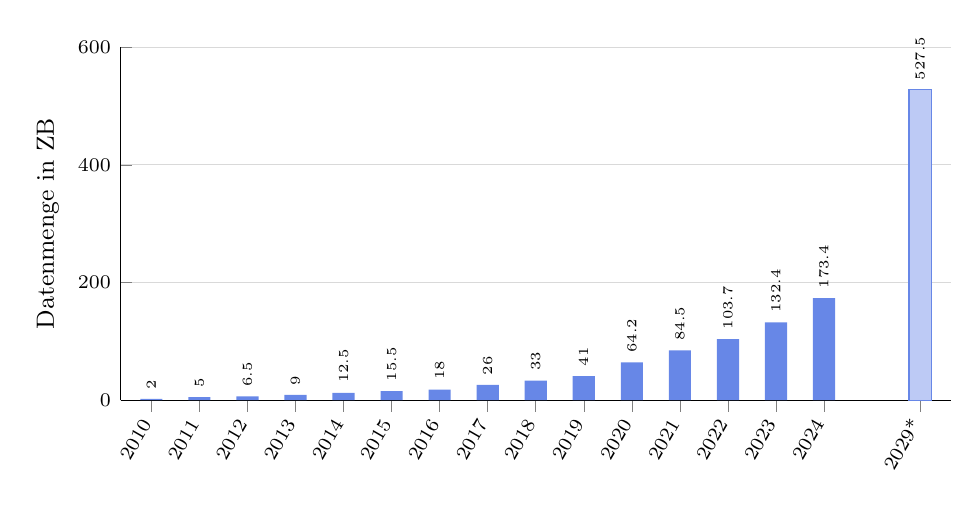
\begin{tikzpicture}
  \begin{axis}[
      width=\linewidth,
      height=.5\linewidth,
      ybar,
      bar width=.8em,
      bar shift=0pt,
      ymin=0, ymax=600,
      ylabel={Datenmenge in ZB},
      % Lücke zwischen 2024 und 2029 als leere Kategorie
      symbolic x coords={2010,2011,2012,2013,2014,2015,2016,2017,2018,2019,2020,2021,2022,2023,2024,gap,2029},
      xtick={2010,2011,2012,2013,2014,2015,2016,2017,2018,2019,2020,2021,2022,2023,2024,2029},
      xticklabels={2010,2011,2012,2013,2014,2015,2016,2017,2018,2019,2020,2021,2022,2023,2024,2029*},
      x tick label style={rotate=60, anchor=east, font=\scriptsize},
      y tick label style={font=\scriptsize},
      ylabel style={font=\small},
      nodes near coords,
      nodes near coords style={font=\tiny, rotate=90, anchor=west},
      point meta=explicit symbolic,
      ymajorgrids, grid style={gray!30},
      axis x line*=bottom, axis y line*=left,
      enlarge x limits=.04,
    ]
    % gemessene bzw. geschätzte Werte bis 2024
    \addplot[fill=RoyalBlue!80, draw=none] coordinates {
        (2010,2) [2] (2011,5) [5] (2012,6.5) [6.5] (2013,9) [9] (2014,12.5) [12.5]
        (2015,15.5) [15.5] (2016,18) [18] (2017,26) [26] (2018,33) [33] (2019,41) [41]
        (2020,64.2) [64.2] (2021,84.5) [84.5] (2022,103.66) [103.7] (2023,132.4) [132.4] (2024,173.4) [173.4]
      };
    % Prognose 2029 (heller dargestellt)
    \addplot[fill=RoyalBlue!35, draw=RoyalBlue!80] coordinates {(2029,527.5) [527.5]};
  \end{axis}
\end{tikzpicture}

  \caption[Entwicklung der weltweiten Datenmenge]{Jährlich weltweit erzeugte, kopierte und genutzte Datenmenge in Zettabyte (2029: Prognose, Werte vor 2024 aus älteren Veröffentlichungen). Daten: IDC, veröffentlicht von Western Digital, zusammengestellt von Statista, \url{https://de.statista.com/statistik/daten/studie/267974/umfrage/prognose-zum-weltweit-generierten-datenvolumen/} (abgerufen am 22.11.2026).}
  \label{fig:daten-global}
\end{figure}

Dies hat zur Folge, dass Datenzentren immer grösser werden und mehr Energie verbrauchen, wie das folgende Video
verdeutlicht: \url{https://youtu.be/_r97qdyQtIk?t=2m14s}

\begin{myexercise}[Bits und Bytes]\label{myexercise:bits-bytes}
  Verwenden Sie \cref{table:groessenordnungen}.
  \begin{aenum}
    \item Wie viele Bit sind ein Kilobyte?
    \item Ein Handyfoto belegt etwa 3 MB. Wie viele solche Fotos haben auf einer Speicherkarte mit 64 GB Platz?
    \item Ordnen Sie der Grösse nach: 2 GB, 1500 MB, 0.001 TB, \num{4000000} kB.
  \end{aenum}
  \begin{myanswer}
    \begin{aenum}
      \item 1 kB $=$ \num{1000} B $=$ $\num{1000}\cdot 8$ bit $=$ \num{8000} bit.
      \item 64 GB $=$ \num{64000} MB, also $\num{64000} : 3 \approx \num{21333}$ Fotos.
      \item 0.001 TB $=$ 1 GB $<$ 1500 MB $=$ 1.5 GB $<$ 2 GB $<$ \num{4000000} kB $=$ 4 GB.
    \end{aenum}
  \end{myanswer}
\end{myexercise}

\subsection{Tabellen}
\label{subsec:tables}
Der allergrösste Teil der oben erwähnten Daten befindet sich in sogenannten Datenbanken. Datenbanken bestehen im Wesentlichen aus Tabellen, weshalb wir im Folgenden zunächst anschauen, wie eine Tabelle aufgebaut ist. Ein Beispiel einer Tabelle ist in \cref{table:cia-values} gegeben.

\begin{table}[H]
  \centering
  \begin{tabular}{lcccc}
    \toprule
    \textbf{Name}    & \textbf{Region} & \makecell{\textbf{Fläche}\\(Tsd. km$^2$)} & \makecell{\textbf{Einwohner}\\(Mio.)} & \makecell{\textbf{BIP}\\(Mrd. USD)} \\
    \midrule
    Afghanistan      & Asien           & 652             & 25.8               & 21.0         \\
    Albanien         & Europa          & 28.7            & 3.49               & 5.6          \\
    Algerien         & Afrika          & 2381.7          & 31.2               & 147.6        \\
    Amerikanische... & Ozeanien        & 0.199           & 0.0654             & 0.15         \\
    Andorra          & Europa          & 0.468           & 0.0668             & 1.2          \\
    Angola           & Afrika          & 1246.7          & 10.1               & 11.6         \\
    Anguilla         & Mittelamerika   & 0.091           & 0.0118             & 0.088        \\
    Antarktik        & Antarktis       & 14000           & 0                  & 0            \\
    Antigua und...   & Mittelamerika   & 0.442           & 0.0664             & 0.524        \\
    Argentinien      & Südamerika      & 2766.9          & 36.9               & 367          \\
    \midrule
    ...              & ...             & ...             & ...                & ...          \\
    \bottomrule
  \end{tabular}
  \caption{Länder-Tabelle}
  \label{table:cia-values}
\end{table}

Eine Tabelle besteht aus Zeilen und Spalten, wie in \cref{table:table-cia} gezeigt.


\begin{table}[H]
  \centering
  \tiny
  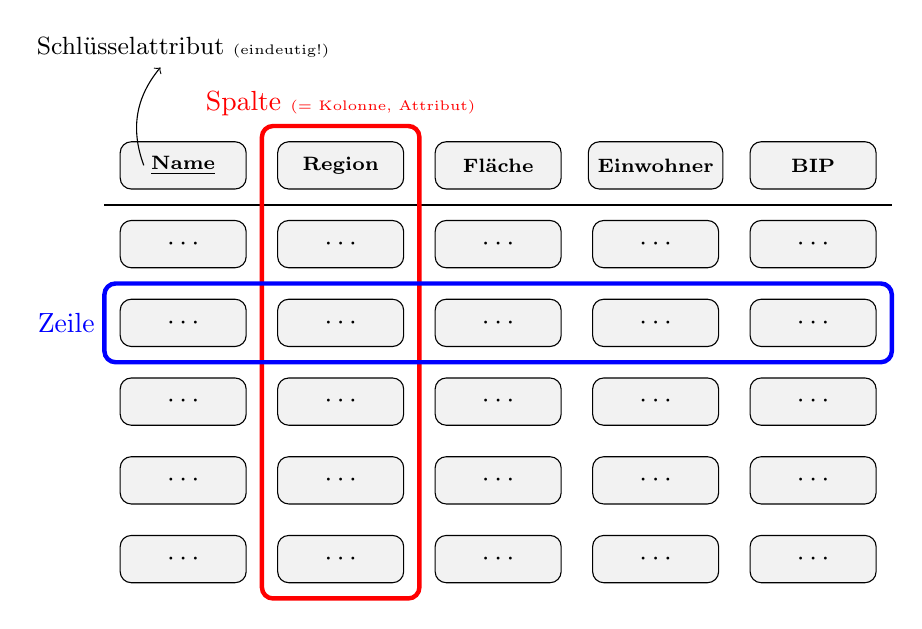
\begin{tikzpicture}
    % Define style for cell
    \tikzstyle{cell} = [draw, rectangle, minimum width=1.6cm, minimum height=.6cm, fill=gray!10, rounded corners]
    \tikzstyle{cellcdot} = [draw, rectangle, minimum width=1.6cm, minimum height=.6cm, fill=gray!0, rounded corners]

    % Draw the table
    \foreach \row in {1,...,6} {
        \foreach \col/\ctitle in {1/\underline{Name},2/Region,3/Fläche,4/Einwohner,5/BIP} {
            \node(\col\row)[cell] at (\col*2, -\row) {
              \ifnum\row=1
                \scriptsize\textbf{\ctitle}\normalsize
              \else
                $\cdots$
              \fi
            };
          }
      }
    \draw[black, thick] (1,-1.5) -- (11,-1.5);

    \draw [red,ultra thick,rounded corners]
    (3,-.5) rectangle (5,-6.5);

    \draw [blue,ultra thick,rounded corners]
    (1,-2.5) rectangle (11,-3.5);

    \node[above] at (4,-0.5){\textcolor{red}{Spalte \tiny($=$ Kolonne, Attribut)\normalsize}};
    \node[left] at (1,-3){\textcolor{blue}{Zeile}};

    \node(label) at (2,.5) {\small Schlüsselattribut \tiny(eindeutig!)};
    \path[->] (1.5,-1) edge[bend left] node [left] {} (label);
  \end{tikzpicture}
  \caption{Typische Tabellenstruktur anhand einer Tabelle mit Informationen zu Ländern}
  \label{table:table-cia}
\end{table}
In \cref{table:table-cia} enthält jede \textcolor{blue}{Zeile} Informationen zu einem Land: dessen Name, die Region (=Kontinent), Fläche, die Einwohnerzahl und das Bruttoinlandprodukt (BIP). In \cref{table:cia-values} ist die Fläche in Tausend km$^2$ angegeben, die Einwohnerzahl in Millionen und das BIP in Milliarden US-Dollar.
Jede \textcolor{red}{Spalte} enthält Informationen desselben Typs, beispielsweise die Regionen aller Länder, die Flächen oder die Einwohnerzahlen.
In einer Spalte sollten also alle Werte denselben Typ haben, beispielsweise \enquote{Zahl} (Fläche, Einwohner, BIP) oder
\enquote{Text} (Name, Region).
Nicht zuletzt gibt es in gewissen Tabellen (genau) ein Schlüsselattribut, dessen Werte eindeutig sein müssen.
Dies bedeutet in \cref{table:table-cia} beispielsweise, dass kein Ländername zweimal oder mehr vorkommen darf. Weshalb dies wichtig ist, werden wir später sehen.

Eine Datenbank ist vereinfacht gesagt eine Sammlung aus mehreren Tabellen, auf die mehrere Geräte zugreifen können (lesen und schreiben), wie in \cref{fig:db-schema} gezeigt.



\begin{figure}[H]
  \centering
  \begin{tikzpicture}
    \tikzstyle{c} = [draw, shape=circle, draw=black!20, fill=black!10]
    \Large
    %\draw[step=1cm,gray,very thin] (-4,-4) grid (4,4);
    \node [circle, draw=black!20, fill=black!10, minimum size=.5cm](db) at (0,0) {\faTable};
    \node [c](l1) at (-3,0) {\emoji{laptop}};
    \node [c](l2) at (-2,-2) {\emoji{desktop-computer}};
    \node [c](l3) at (0,-3) {\emoji{laptop}};
    \node [c](l4) at (2,2) {\emoji{desktop-computer}};
    \node [c](l5) at (0,3) {\emoji{laptop}};
    \node [c](l6) at (3,0) {...};
    \node [c](mp1) at (2,-2) {\emoji{mobile-phone}};
    \node [c](mp2) at (-2,2) {\emoji{mobile-phone}};


    \foreach \nodeN in {l1,l2,l3,l4,l5,l6,mp1,mp2}{
        \path[->, red] (db) edge[bend right=10] node [left] {} (\nodeN);
        \path[->, blue] (\nodeN) edge[bend right=10] node [left] {} (db);
      }

  \end{tikzpicture}
  \caption{Geräte können Daten an die Datenbank \textcolor{blue}{senden} und von ihr \textcolor{red}{empfangen}}
  \label{fig:db-schema}
\end{figure}

Datenbanken und Tabellen finden Anwendung in allen möglichen Bereichen des täglichen Lebens:
\begin{itemize}
  \item \textbf{Social Media}: Instagram, TikTok, LinkedIn, etc.
  \item \textbf{Shopping}: Galaxus, AliExpress, etc.
  \item \textbf{Netzwerke}: SBB, swissgrid (Strom-Netzwerk), etc.
\end{itemize}

Wie können wir mit den riesigen Datenmengen umgehen und sinnvolle Einsichten daraus gewinnen?

Eine der verbreitetsten Arten, Tabellen und Datenbanken zu erstellen, zu verändern und zu analysieren, ist die Programmiersprache \gls{SQL}. Im Folgenden verwenden wir die Datenbanken aus der Lern-Plattform InstaHub, um uns mit \gls{SQL} vertraut zu machen.

Alle Beispiele können direkt auf InstaHub ausgeführt werden. Die \textcolor{Plum}{\textbf{Abgaben}} sind violett markiert
und befinden sich auf Moodle unter \enquote{Quiz \gls{SQL}}.


\clearpage
\begin{myexercise}[Einrichtung von InstaHub \emoji{camera-with-flash}]\label{myexercise:instahub-setup}
  \begin{table}[H]
    \centering
    \begin{tabular}{r|l}
      \emoji{chequered-flag} & Selber eine Datenbank administrieren \\\hline
      %\emoji{family-man-woman-girl-boy} & 3er- bis 4er-Gruppen \\\hline
      \emoji{student}        & Einzelarbeit                         \\\hline
      \emoji{stopwatch}      & ca. 25 min.
    \end{tabular}
  \end{table}

  Führen Sie folgende Schritte aus:\par

  \begin{enumerate}
    \item Auf \url{https://instahub.org} gehen
    \item Auf Hub erstellen (rechts oben) klicken und einen Hub erstellen.
          \begin{figure}[H]
            \centering
            \includegraphics[width=1.5cm]{Grundlagen_Info/06_Datenbanken/Figures/tutorial-instahub-1}
          \end{figure}
    \item Geben Sie folgende Angaben ein (siehe Bild unten):
          \begin{itemize}
            \item Name der Lehrperson (klein geschrieben und ohne Abstände): \texttt{cyrilblum} oder \texttt{thomasgraf}
            \item Der Username lautet \texttt{admin} und kann nicht geändert werden.
            \item Ihren Namen und Ihr Passwort können Sie frei setzen.
            \item Sie können entweder eine echte E-Mail-Adresse angeben oder die generierte E-Mail-Adresse so lassen.
              Im zweiten Fall können Sie jedoch Ihr Passwort nicht mehr per Mail zurücksetzen, falls Sie dieses je verlieren sollten.
            \item Geben Sie mir mündlich Bescheid, dass Sie die Seite erstellt haben. Wir müssen Ihren persönlichen Hub ($=$ Ihre Webseite) manuell aktivieren. Dies dauert nur wenige Sekunden.
          \end{itemize}
          \begin{figure}[H]
            \centering
            \includegraphics[width=.8\textwidth]{Grundlagen_Info/06_Datenbanken/Figures/tutorial-instahub-2}
          \end{figure}
    \item Merken oder notieren Sie sich Ihr Passwort an einem sicheren Ort.
    \item Sie haben nun eine eigene Webseite unter \url{https://[meinefarbeXX].instahub.org}, wobei \texttt{[meinefarbeXX]} durch Ihre Farbe ersetzt werden muss (siehe Bild oben).
    \item Sie können sich jetzt auf Ihrer individuellen Webseite mit dem Benutzernamen \texttt{admin} (\textit{nicht} Ihrer E-Mail-Adresse) und dem von Ihnen zuvor gewählten Passwort anmelden.
      Sie sind nun als \textcolor{RoyalBlue}{AdministratorIn} Ihres eigenen sozialen Netzwerks eingeloggt.
  \end{enumerate}
\end{myexercise}

\begin{myexercise}
  Schreiben Sie sich den Namen Ihrer InstaHub-Seite auf, also z.B.
  \begin{center}
    \url{https://[meinefarbeXX].instahub.org},
  \end{center}
  wobei \texttt{[meinefarbeXX]} durch Ihre Farbe ersetzt werden muss!
  Laden Sie diesen auf Moodle unter \enquote{Name InstaHub} hoch, so dass Sie den Link auf Ihr InstaHub später einfach wieder finden.
\end{myexercise}

\begin{myexercise}[Inbetriebnahme von InstaHub]
  \begin{table}[H]
    \centering
    \begin{tabular}{r|l}
      \emoji{chequered-flag}        & Lernen, mithilfe von \gls{SQL} eigene Abfragen zu machen \\\hline
      \emoji{family-man-woman-girl} & 2er- bis 3er-Gruppen                                      \\\hline
      \emoji{stopwatch}             & ca. 60 min.
    \end{tabular}
  \end{table}
Bestimmen Sie eine Person pro Gruppe, die sich auf der eigenen Webseite mit dem Benutzernamen \texttt{admin} und dem von Ihnen
gewählten Passwort anmeldet. Ihre eigene Webseite ist:

\url{https://meinefarbeXX.instahub.org}

Wobei \texttt{[meinefarbeXX]} durch Ihre Farbe ersetzt werden muss.

Die anderen Personen der Gruppe lesen \cref{ch:abfragen} aus diesem Skript und helfen der
ersten Person dabei, die \gls{SQL}-Befehle zu schreiben.

  Sie können jetzt unter folgendem Menüpunkt Ihre eigene Datenbank administrieren:

  \begin{figure}[H]
    \centering
    \includegraphics[width=.9\textwidth]{Grundlagen_Info/06_Datenbanken/Figures/instahub-SQL}
  \end{figure}
  Als Erstes sehen Sie eine Liste der verfügbaren Tabellen sowie der dazugehörigen Spaltennamen (siehe Bild unten).
  Tabellennamen sind in \textcolor{orange}{Orange}, Spaltennamen in \green{Grün} markiert.
  \begin{figure}[H]
    \centering
    \includegraphics[width=.9\textwidth]{Grundlagen_Info/06_Datenbanken/Figures/instahub-tables}
    \caption{Die Tabellen von InstaHub und deren Attribute}
    \label{fig:tables-instahub}
  \end{figure}
\end{myexercise}

\newpage
